\section{Методология}

Целью работы было получить размеченный корпус и обученную модель, извлекающую именованные сущности. После обзора литературы были намечены задачи и работа была предварительно разделена на несколько этапов.

\begin{enumerate}
\item Получение и разметка данных
\item Выбор, обучение и тюнинг моделей
\item Сравнение результатов
\end{enumerate}

Но в течение работы были внесены корректировки. Во-первых, как я упоминала ранее в обзоре литературы, с представленными результатами в статье Невзоровой невозможно сравниваться, поскольку цели моей и их работ различаются. Во-вторых, качество полученных данных оказалось не лучшим из возможных, а алгоритм Невзоровой, разработанный как раз для разметки данных, мог бы улучшить имеющийся корпус, используемый для обучения моделей. Как следствие, было принято решение воспроизвести алгоритм из статьи Невзоровой и воспользоваться полученными результатами для разметки данных.

\begin{enumerate}
\item Получение и конвертирование данных в нужный формат.
\item Выбор, обучение и тюнинг моделей
\item Воспроизведение статьи Невзоровой
\item Разметка данных с помощью алгоритма Невзоровой
\item Обучение и тюнинг моделей
\item Сравнение результатов
\end{enumerate}


\section{Получение и разметка данных}

\subsection{Туган Тел}

Обзор литературы показал, что существует корпус татарских текстов Туган Тел\cite{tugan_tel}. Данный копрус имеет также свою систему <<корпус-менеджер>>, которая представлена в виде сайта. На этом сайте можно искать по словоформе или лемме с огромным количеством параметров [\ref{fig:tugan_tel_1}], однако возможности просто скачать весь корпус не оказалось. Я предполагаю, что у Академии наук Республики Татарстан есть API для исполнения запросов на большом количестве данных и в каком-то более удобном формате, чем запрос на сайте, но у меня доступа к такому ресурсу нет. 

\begin{figure}
\caption{Параметры на сайте \href{http://tugantel.tatar/}{tugantel.tatar} для поиска по корпусу}
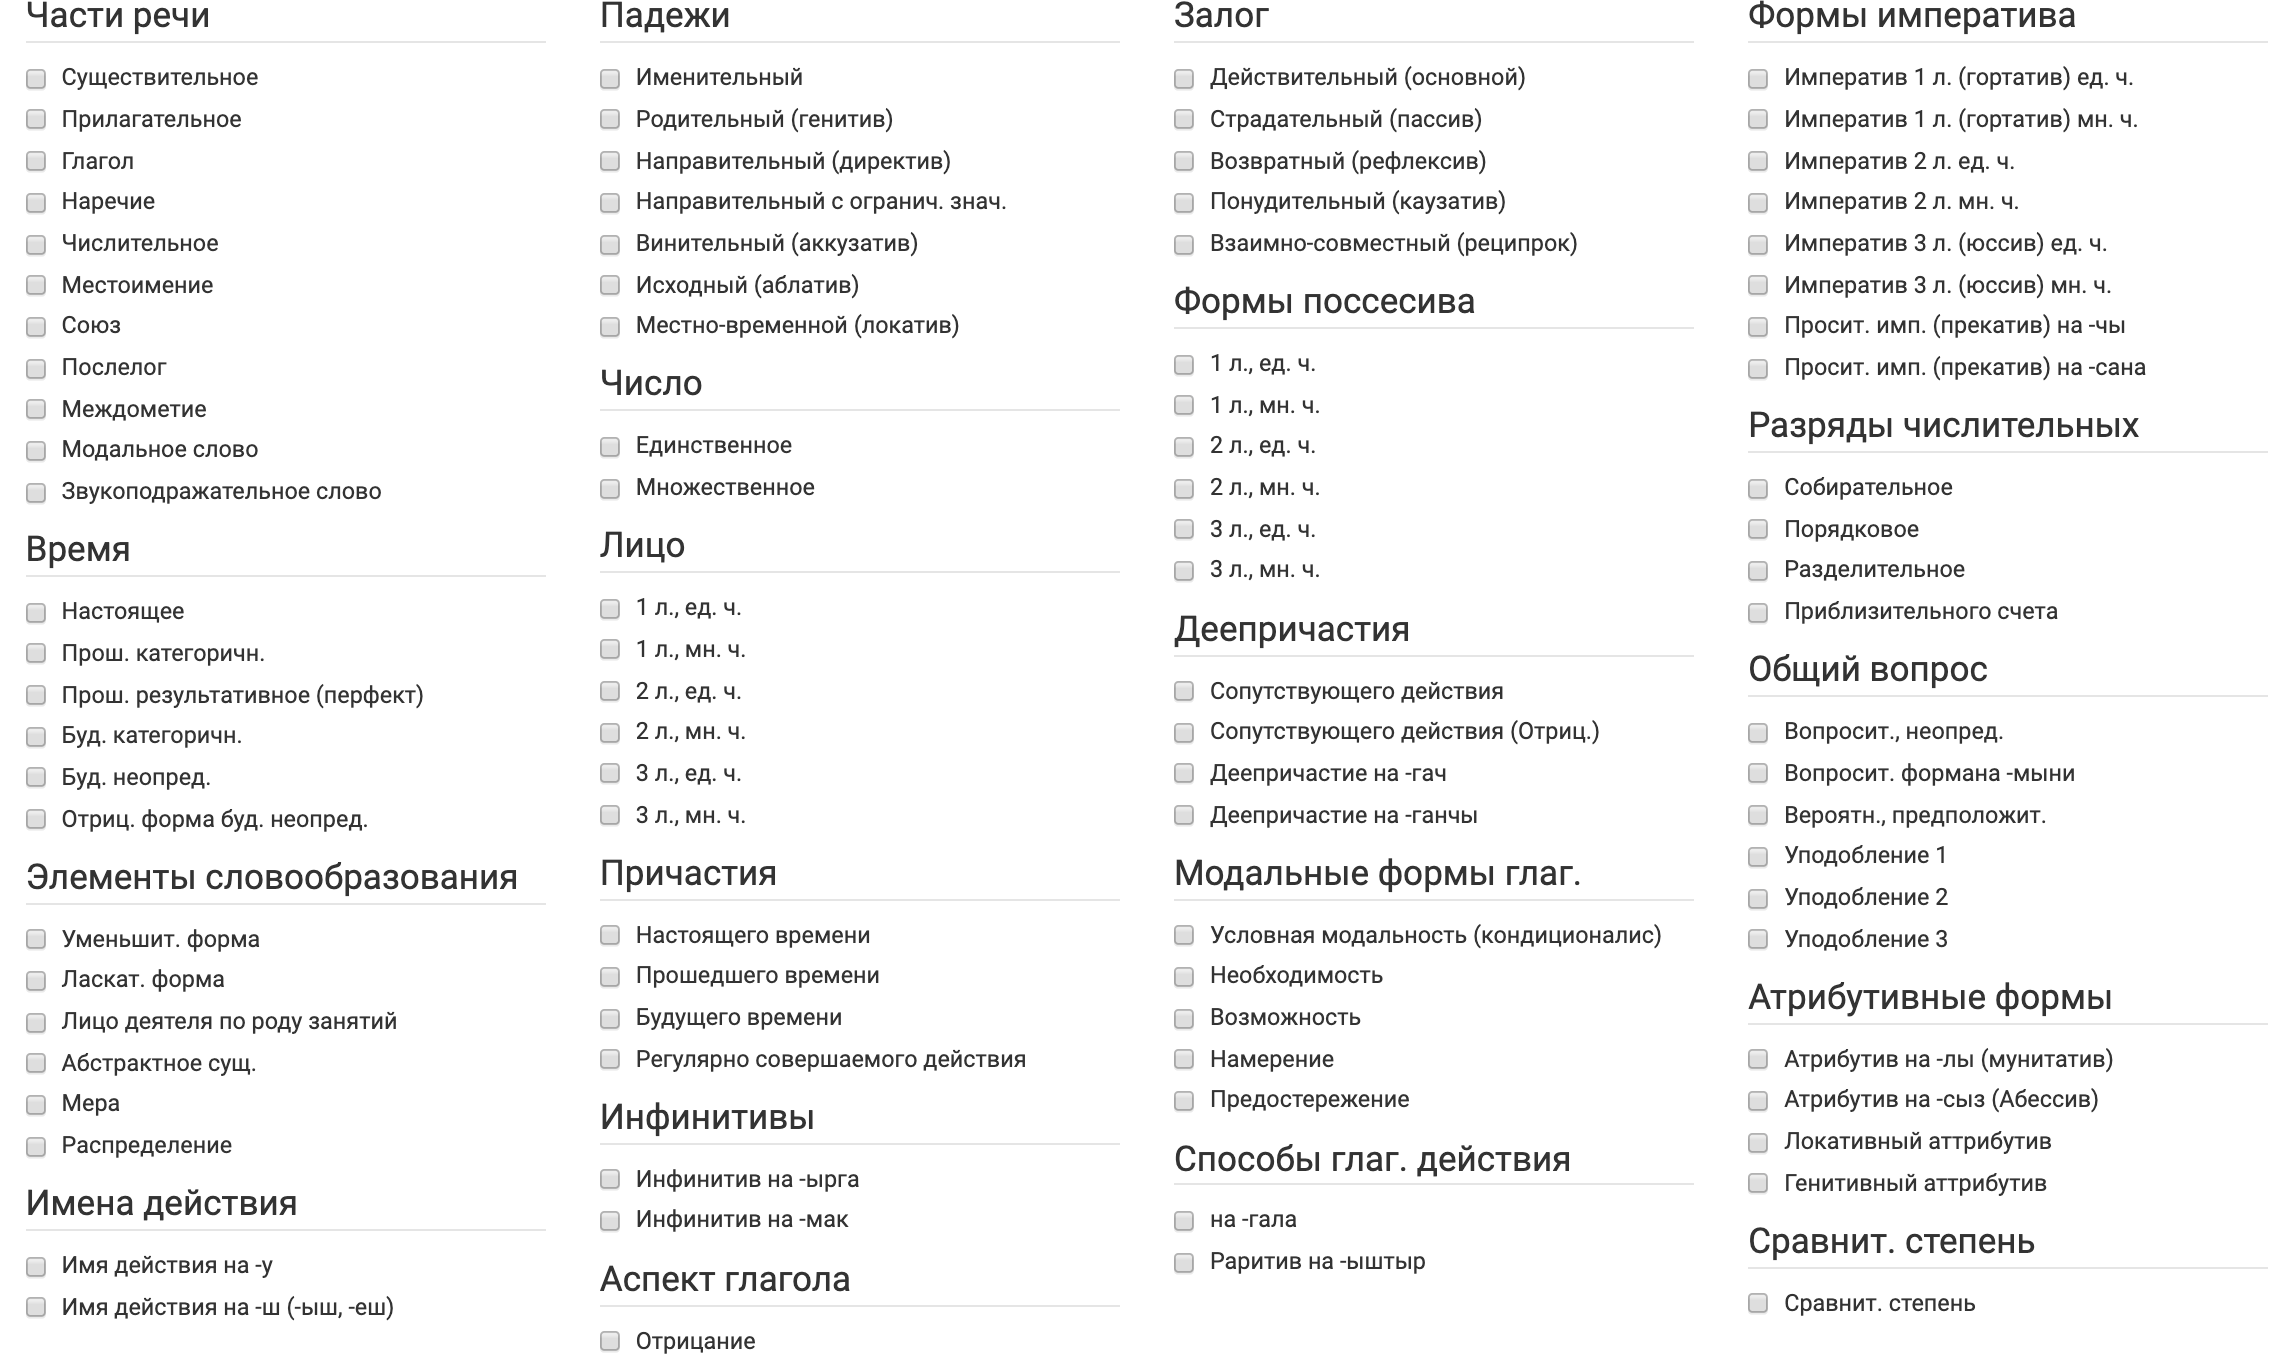
\includegraphics[width=\textwidth]{tugan_tel_1}
\label{fig:tugan_tel_1}
\end{figure}


Я связалась с Невзоровой по указанной в статье электронной почте, чтобы узнать подробности об их работе и попросить о сотрудничестве. Невзорова ответила на моё письмо и предоставила мне доступ к корпусу. В предоставленном мне корпусе было ~30 млн словоформ, а не ~194 млн, как заявлено на сайте. 

Корпус представляет из себя .zip файл, состоящий из $7557$ .txt файлов, в общей сложности весом $1\ 183\ 023\ 978$ Б. Как уже упоминалось ранее, корпус Туган Тел автоматически размечен с помощью программного инструментарии PC-KIMMO. Разметка выглядит следующим образом (см. рис \ref{fig:sample_sent}). На нечетной строке написано слово, на следующей --- разметка слова. Знаки препинания тоже являются <<словами>>. Существует проблема с разделением текста на предложения, так как не существует никакой специальной разметки для окончания предложений. Было принято решение разделять предложения по точкам, даже если это не самый точный способ разбиения.

\begin{figure}
\caption{Пример случайного предложения из корпуса Туган Тел}
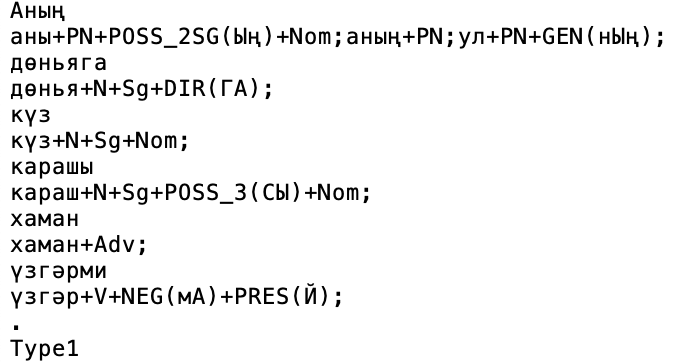
\includegraphics{sample_sent}
\label{fig:sample_sent}

Перевод: Его мировоззрение никогда не меняется.
\end{figure}

Со всеми тегами морфоанализатора можно ознакомиться на сайте \href{http://tatmorphan.pythonanywhere.com/morphan_tags}{tatmorphan.pythonanywhere.com}.

В тегах морфоанализатора присутствует тег PROP, который обозначает имена собственное. Для первой итерации было решено считать имена собственные именованными сущностями. Как можно заметить в примере на рис. \ref{fig:prop_sent}, в корпусе имена собственные иногда бывают с маленькой буквы, что говорит о том, что данные содержат в том числе и ошибки.
Всего в текстах 30 753 824 слов, из них 534 514 это слова с атрибутом PROP, что составляет $1,7\%$ от всех слов. 

\begin{figure}
\caption{Пример предложения из корпуса Туган Тел с атрибутом PROP}
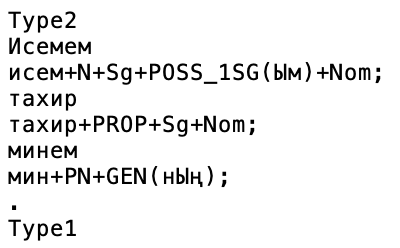
\includegraphics{pics/prop_sent}
\label{fig:prop_sent}

Перевод: Тахир меня зовут.
\end{figure}

\subsection{Татарская Википедия}

Кроме корпуса <<Туган Тел>> другого большого количества текстов, собранных в одном месте, найдено не было, поэтому было принято решение скачать википедию на татарском языке.

На данный момент татарская википедия содержит $89\ 252$ статей, которые написаны как с помощью кириллической, так и с помощью латинской письменности. Данный раздел Википедии был открыт 15 сентября 2003 года и сначала функционировал исключительно на латинице, позже статьи писались с использование обоих алфавитов; сейчас же достигнут консенсус об использовании единой системы категорий на кириллице, однако некоторые статьи до сих пор остаются латинизированными (примерно треть от всех имеющихся статей). Причин такой путаницы несколько. 

Во-первых, проблема алфавита в татарском языке стояла ещё со времен Советского Союза, т.к. до 1927 года использовалась арабская письменность, с 1927-1939 --- латинская письменность, а 5 мая 1939 года Президиум Верховного Совета Татарской АССР принял указ <<О переводе татарской письменности с латинизированного алфавита на алфавит на основе русской график>> и начал использоваться кириллический алфавит. Поскольку переход на другую письменность происходил принудительно, до сих пор ведутся дебаты о возвращении на латинский алфавит. На текущий момент в республике Татарстан кириллица остаётся официальным алфавитом, однако стало допустимым использование латиницы и арабицы при обращении граждан в государственные органы и латиницы при транслитерации. Существует официальное соответствие данных трёх алфавитов.

Во-вторых, в 2000-x годах существовала проблема с записью текстов на компьютере, вызванная отсутствием букв дополнительной кириллицы в стандартных раскладках.

В связи с этим статьи на латинице пришлось конвертировать в кириллицу и в то же время случайно не перевести английские названия (например, ссылки). Данная процедура была проведена с помощью автоматического скрипта, поэтому возможны артефакты в виде, например, слова <<хттп>>.

\begin{figure}[H]
\begin{minipage}{\textwidth}
\caption{Статья <<Камский бассейновый округ>>}
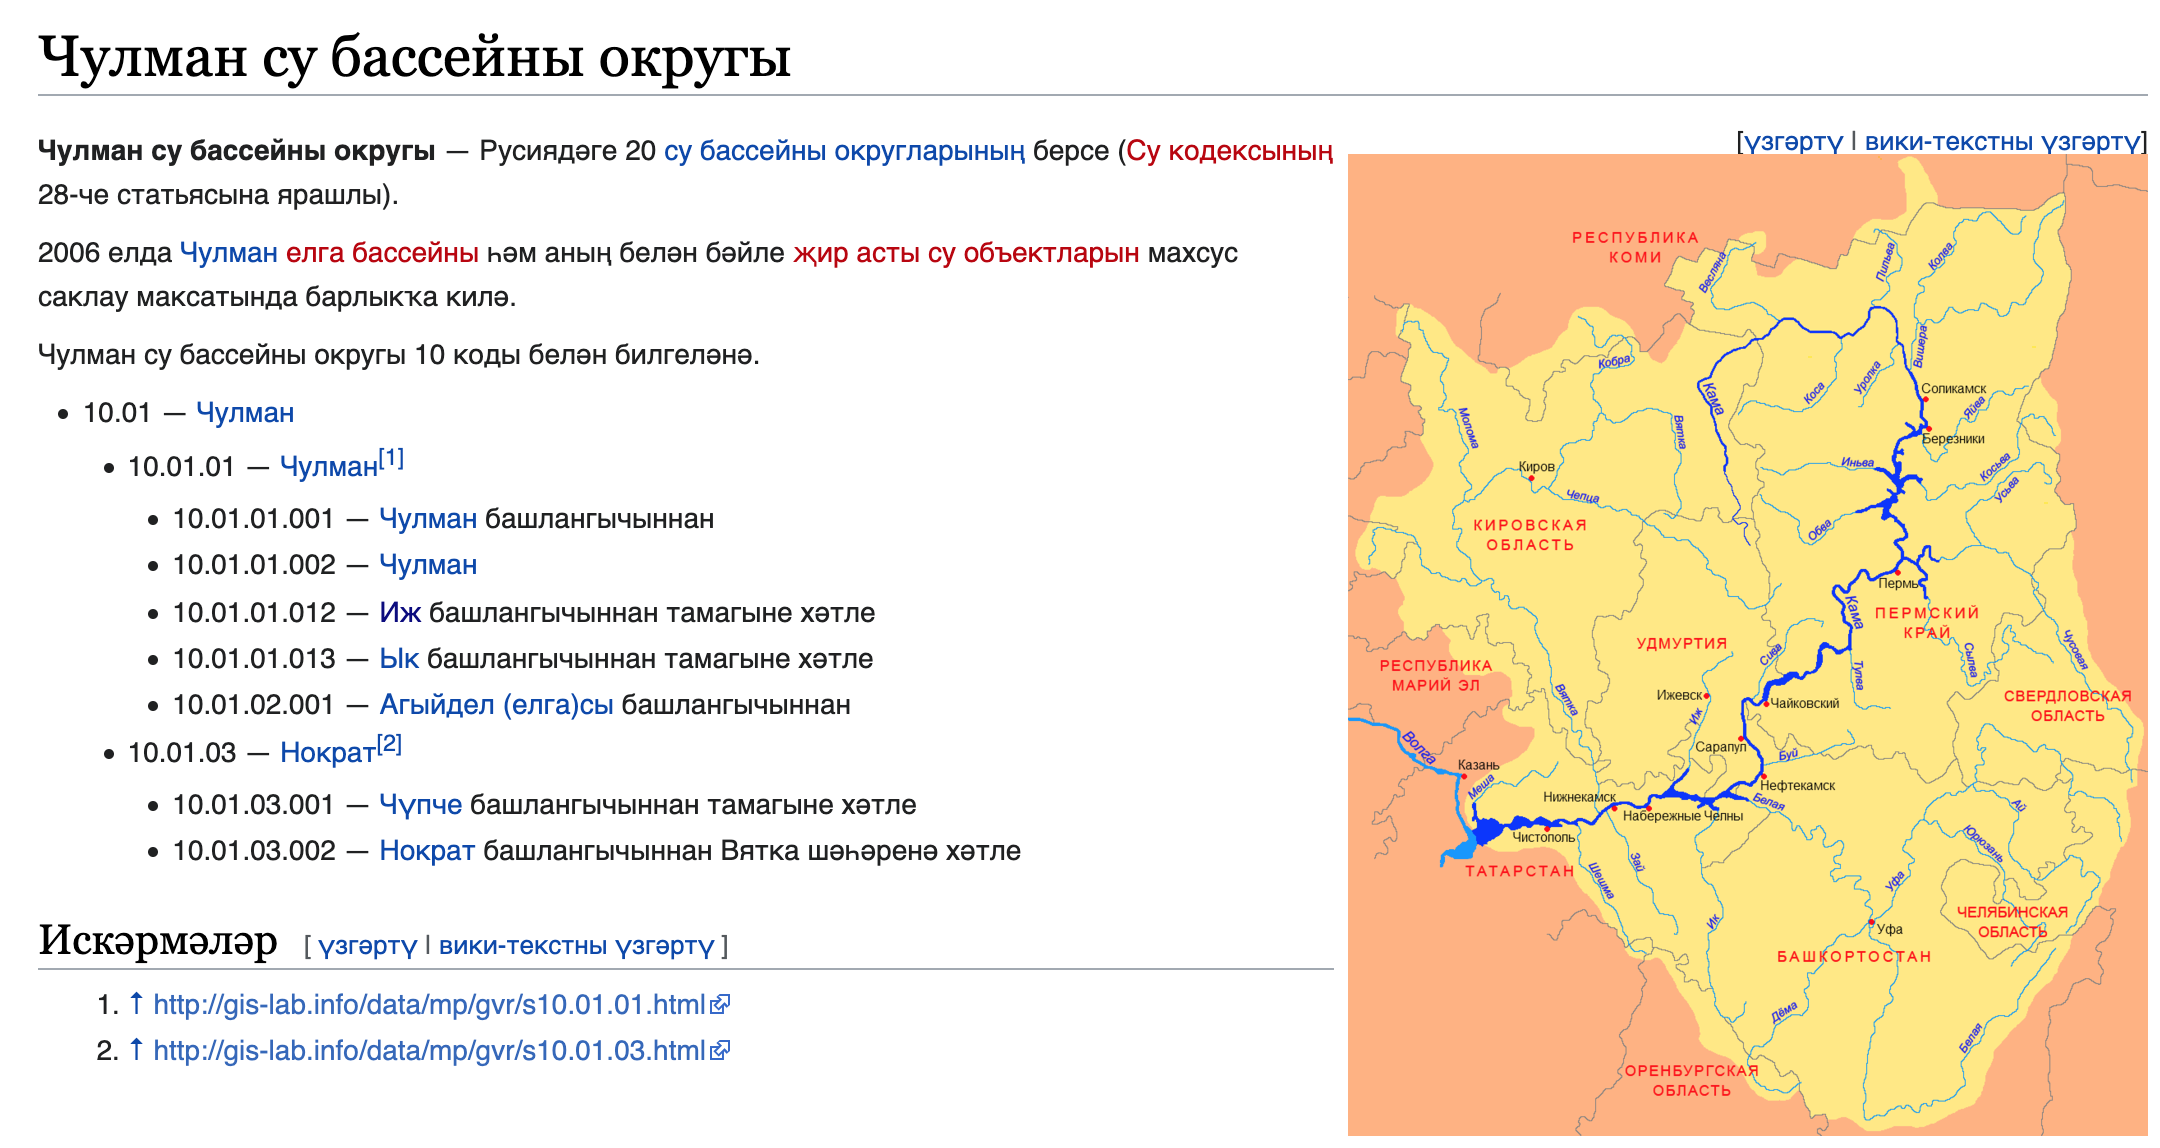
\includegraphics[width=\textwidth]{bassein_article}
\label{fig:bassein_article}
\end{minipage}

\begin{minipage}{\textwidth}
\caption{Пример сгенерированных статей из Википедии}
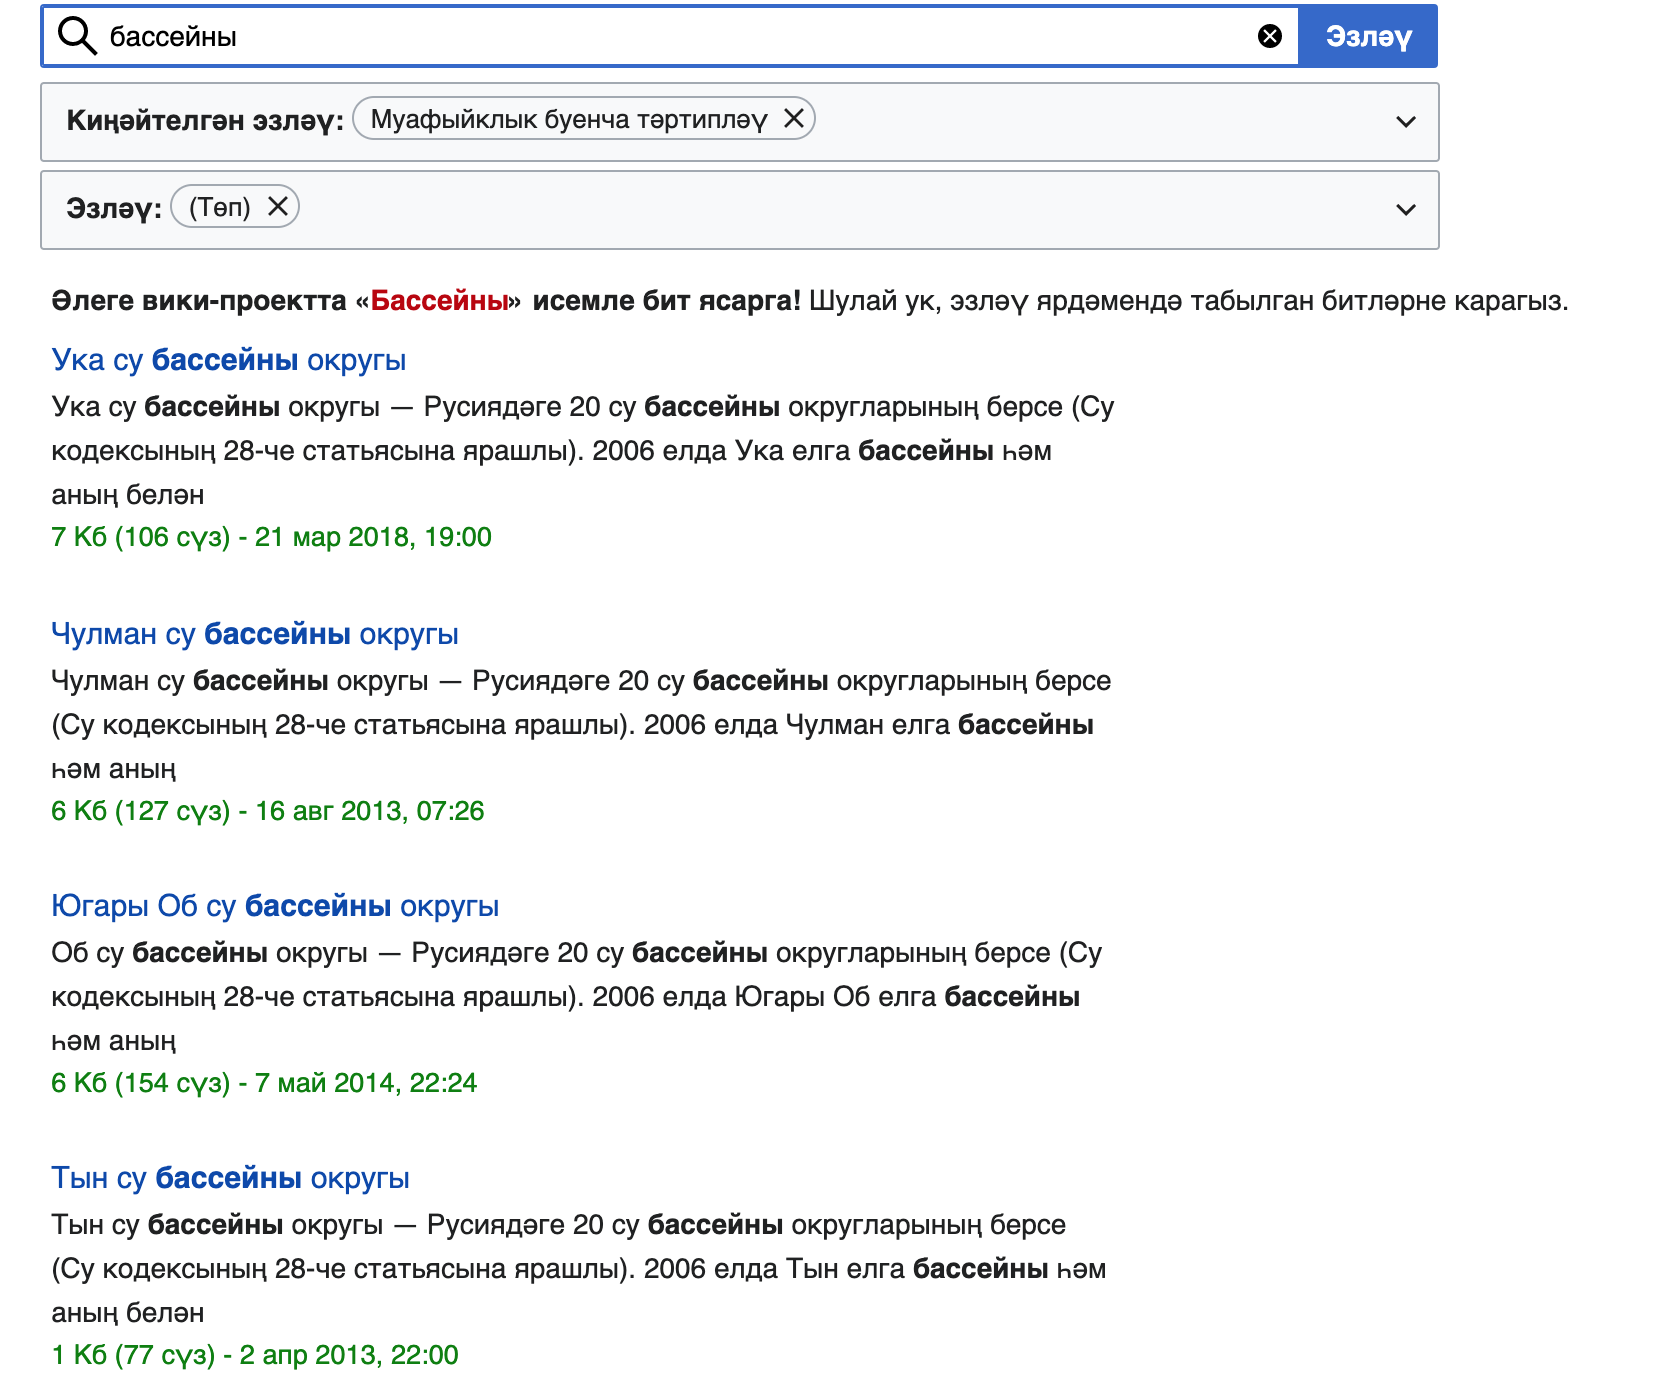
\includegraphics[width=\textwidth]{bassein_search}
\label{fig:bassein_search}
\end{minipage}
\end{figure}


Также важно отметить, что википедия представляет из себя набор статей, написанных в академическом стиле, что не вполне отображает разнообразие языка в различных сферах употребления; в этом аспекте Туган Тел гораздо лучше. В Википедии в том числе существуют автоматически сгенерированные статьи, это ухудшает качество текстов как корпуса для обучения, так как некоторые фразы становятся частотными не из-за того, что они действительно часто используются в языке, а из-за множества сгенерированных статей. Например, статьи про бассейновые округа (<<бассейны>> это не множественное число слова <<бассейн>>, а принадлежность к третьему лицу). Статья про Камский бассейновый округ (рис. \ref{fig:bassein_article}) и по тому же шаблону ещё много других статей про бассейновые округа (рис. \ref{fig:bassein_search}).

Справедливости ради следует заметить, что в русской википедии они тоже сгенерированны автоматически.

\subsection{Разметка данных для обучения}

Первой итерацией было использование разметки PROP в корпусе Туган Тел, никакие другие теги морфоанализотора не использовались; Википедия не использовалась. 

Во второй итерации использовался воспроизведенный алгоритм Невзоровой, в качестве исходного корпуса для которого применялась Википедия. На данных из Википедии был получен список n-грамм \footnote{Список n-грамм, обозначающих именованные сущности, предоставлен на github.com/ksemiya/NER\_in\_Tatar}, обозначающих именованные сущности по классам PER (персона), LOC (географический объект), ORG (организация) и MISC (всё остальное, но в основном названия языков) С помощью полученного списка была размечена Википедия с помощью сравнения n-грамм на точное равенство, в то время как Туган Тел никак не использовался при данной разметке и был отложен в качестве данных для оценивания.

Для разметки BIO был написан небольшой скрипт, с помощью которого вы можете также получить размеченные данные на своей локальной машине.


\subsection{Разметка данных для оценивания}

Автоматическая разметка не подходит для оценки результатов. Поэтому для оценивания воспроизведенного алгоритма Невзоровой и обученных моделей было принято решение разметить некоторое количество предложений вручную, в силу имеющихся знаний татарского языка. Предложения были выбраны из корпуса Туган Тел из соображений наличия в них хотя бы одной именованной сущности; для этого был использован алгоритм Невзоровой и если он определил наличие именованной сущности, то предложение добавлялось в список кандидатов на ручную разметку. Из полученного списка кандидатов предложения выбирались случайным образом, разметка алгоритмом Невзоровой удалялась до начала ручной разметки, чтобы не влиять на конечный результат. Получился тестовый набор данных golden-bio.txt \footnote{golden-bio.txt также предоставлен на github.com/ksemiya/NER\_in\_Tatar}, основанный на предложениях из корпуса Туган Тел (369 предложений).

\subsection{Проблемы с разметкой данных}

Как было описано и в статье Невзоровой, где исследователи глазами просматривали полученные результаты, отсеивали некорректные и улучшали свой алгоритм с помощью фильтров, так и в моей работе разметка данных происходила итеративно. Например, генерация статей про бассейны в Википедии была как раз выявлена в просмотре полученных результатов после разметки. Также выявлялись пробелы в алгоритме, например, некоторые географические названия, которые не попадали в список, были добавлены позже вручную. Для разметки тегом PER был использован справочник имён. Подводя итог, лучшей всё равно остаётся ручная разметка, а любая автоматическая разметка требует просмотра и последующей корректировки, возможно в несколько этапов, и это занимает очень много времени. С другой стороны, ручная разметка корпуса заняла бы ещё больше время.

\section{Обучение и тюнинг моделей}

\subsection{BiLSTM-CRF}

Была использована модель BiLSTM-CRF из статьи <<A Neural Layered Model for Nested Named Entity Recognition>> \cite{ju-etal-2018-neural}. Она использует разметку BIO, как и многие другие модели для извлечения именованных сущностей. Архитектура модели изображена на рис. \ref{BiLSTMCRF}

\begin{figure}[H]
\caption{Архитектура модели BiLSTM-CRF, рис. из статьи \cite{ju-etal-2018-neural}}
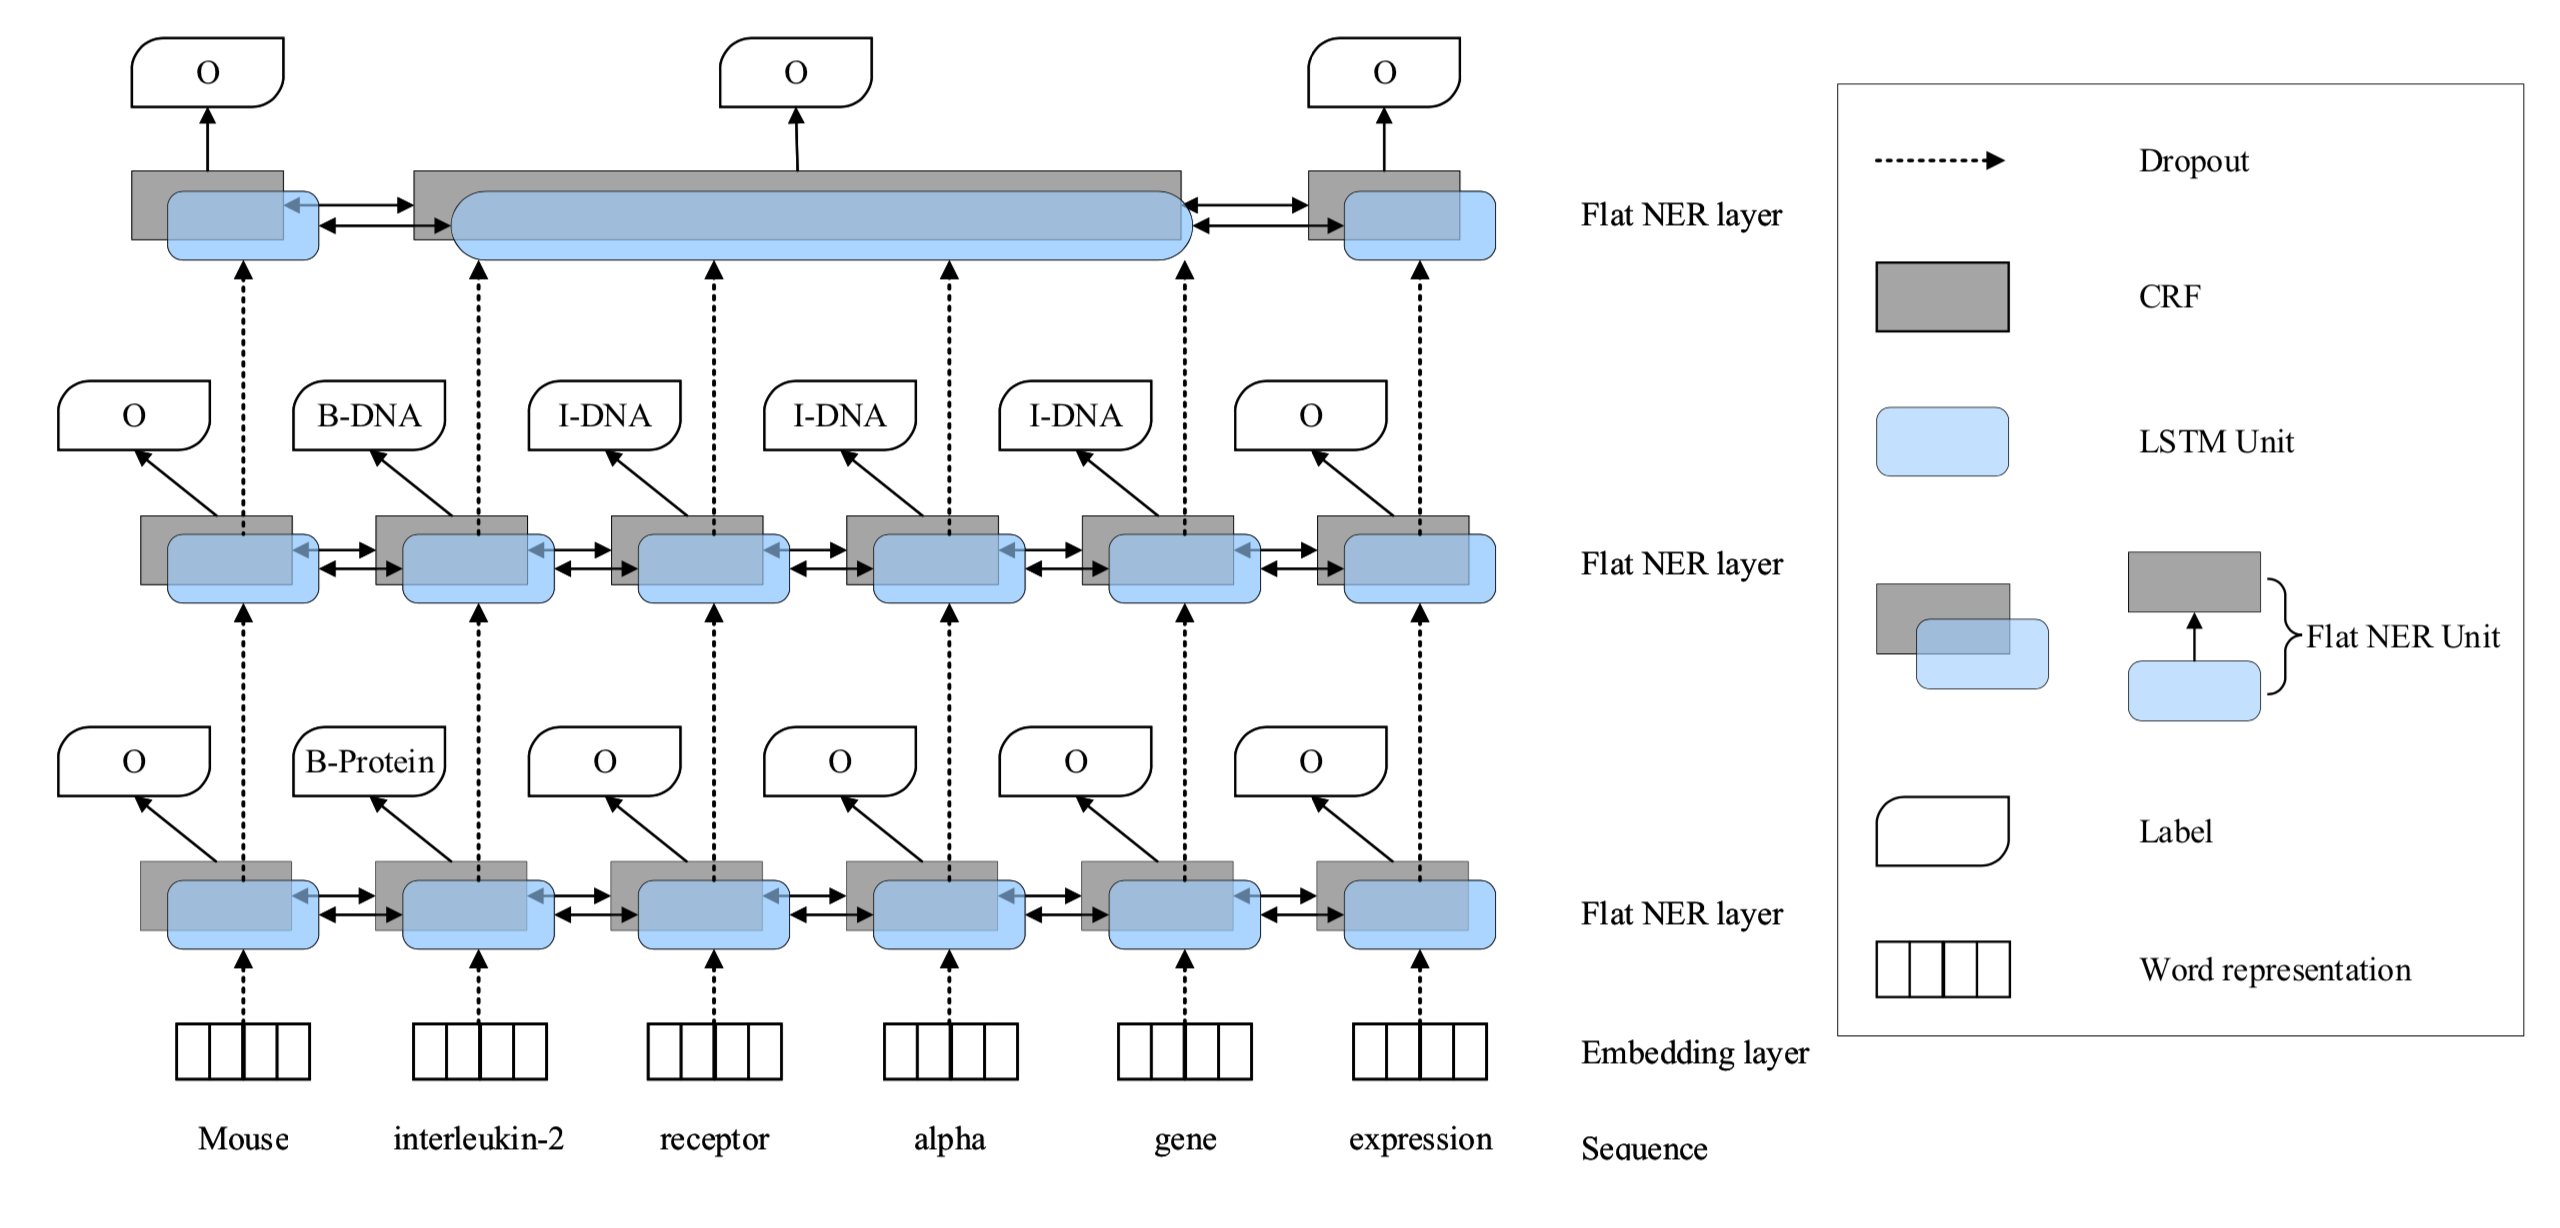
\includegraphics[width=\textwidth]{BiLSTMCRF}
\label{fig:BiLSTMCRF}
\end{figure}


Была возможность запустить модель только на локальной не очень мощной машине, поэтому пришлось обучаться не на всех данных, а только на части.

Первая итерация на данных Туган Тел, где тег PROP стал соответствовать тегу B-PER.

Результат обучения, в данных два тега: O и B-PER.


\medskip

\begin{tabular}{| l | l | l | l | l | l | l |}
\hline
Category               & Precision  &   Recall   &  F-score   \\

\hline
 PER                                 & 99.768     & 90.727     & 95.033      \\
\hline
\end{tabular}


Была сделана демонстрация работы модели в виде сайта, запускающегося на локальной машине, но самые простые примеры не из тестового набора выявили большие несовершенства данной модели --- она не извлечела именованные сущности в самых простых предложениях, поэтому в итоге было принято решение в целом отказаться от её использования. %TODO скриншот
Как можно понять, цифры выше показывают возможность модели обучаться на данных (и модель действительно обучается хорошо, выборка разделяется на тестовую и валидационную и всегда показывает хороший результат), но проблема в том, что сами данные очень низкого качества --- и эту проблему модель, увы, исправить не может.


\subsection{BERT}

\cite{DBLP:journals/corr/abs-1810-04805} Одна из самых известных моделей на сегодняшний день, показала лучшие результаты на классических данных CoNLL 2003 (см. обзор литературы).

Для решения моей задачи была использована библиотека Hugging face \cite{Wolf2019HuggingFacesTS} и претренированная модель bert-base-multilingual-cased, которая обучена на чувствительных к регистру данных из 104-х наибольших Википедий. Данная модель включает в себя и татарский язык (беглый взгляд по токенам показал, что действительно есть как и кириллические, так и латинские токены на татарском языке). 

При обучении модели возникли проблемы с размером корпуса данных. Из-за особенностей реализации обучения модели BERT в HuggingFace, библиотека не была способна сохранить все признаки полностью. Особенность была связана с реализацией загрузки данных в библиотеке. Ей нужно было сохранить все данные в виде признаков PyTorch. Обучение удалось произвести только лишь на $1/3$ всех доступных данных.

Результат обучения, в данных два тега: O и PROP.

\medskip

\begin{tabular}{| l | l | l |}
\hline
Precision  &   Recall   &  F-score     \\

\hline
97.447     & 94.585    & 95.995        \\
\hline
\end{tabular}

Один в один повторение истории с BiLSTM-CRF --- сами по себе цифры очень многообещающие, модель обучилась прекрасно, но на деле они показывают всего лишь натренированность модели на плохих начальных данных, которая в итоге не работает на простых примерах, придуманных из головы. Было принято решение от этой модели отказаться. %TODO скриншот

Вторая итерация обучения была произведена на Википедии, размеченной с помощью списка n-грамм, полученных с помощью алгоритма Невзоровой. В тренировочном наборе были оставлены только те предложения, где есть хотя бы одна именованная сущность.

Результат обучения, в данных 9 тегов:
B-LOC
B-MISC
B-ORG
B-PER
I-LOC
I-MISC
I-ORG
I-PER
O

\begin{tabular}{| l | l | l |}
\hline
Precision  &   Recall   &  F-score     \\

\hline
88.853    & 92.377    & 90.581        \\
\hline
\end{tabular}
 

Как видно, результаты заметно ухудшились, что неудивительно, ведь классов стало в $4.5$ раза больше.

Однако все эти результаты всего лишь показывают, как хорошо модель обучилась предсказывать результаты на имеющихся данных. Чтобы проверить её реальную способность извлечеть именованные сущности, необходимо проверить предсказания на <<золотых>> данных, размеченных вручную, про которые мы с высокой точностью знаем, что они правильные.


\section{Воспроизведение алгоритма из статьи Невзоровой}

Было принято решение воспроизвести алгоритм из статьи Невзоровой и др. \cite{Nevzorova} по двум причинам.

\begin{enumerate}
\item Чтобы была возможность сравнивать результаты.
\item Чтобы разметить данные эффективно и, по возможности, хорошо.
\end{enumerate}

%Обе цели были достигнуты и теперь я имею возможность рассказать вам о проблемах, с которыми я столкнулась во время работы и результатах, полученных в итоге.

Воспроизводить алгоритм по описанию в статье было нетривиально, поэтому, если будут желающие воспроизвести его ещё раз, то я рекомендую описание, которое я дала выше в разделе обзор литературы.

Как было сказано ранее, у меня не было доступа к менеджер-системе Туган Тел \cite{tugan_tel}, поэтому воспроизвести алгоритм в точности не удалось. Попытка приблизиться к результату состояла в том, чтобы использовать в качестве начального слова все возможные словоформы слова, а не только слово само, т.е. частично сделать работу морфоанализатора вручную. Однако возможность делать запросы по каким-то специфичным параметром не была реализована в силу сложности.

Несмотря на все вышеописанные трудности, алгоритм сработал достаточно хорошо, хотя и, как и сказано в работе Невзоровой и др., требовалась значительная ручная чистка полученных данных.

Ручная чистка состояла в просмотре полученных именованных сущностей и исправление по-возможности  не точечно, а <<широкими мазками>> --- добавлением новых начальных слов для поискового запроса или удалением всех очевидно некорректных n-грамм одним вызовом команды grep. Например, по слову <<министрлыгы>> (министерство) появилось множество n-грамм, которые начинались с союза <<һәм>> (и). Это некорректные n-граммы, но удалить их все было достаточно легко. 

Также помимо слов, представленных в работе Невзоровой и др. в качестве начальных, были использованы и другие слова, такие как географические объекты: <<елга>> (река), <<шәһәр>> (город), <<авылы>> (село), <<өлкәсе>> (область) и др., организации:  <<академиясы>> (академия), <<идарә>> (администрация), <<институты>> (институт) и др., персоны: <<абый>> (старший брат), <<апа>> (старшая сестра) и др. (в татарском языке принято называть родственников, например, Ильдар абый, Сания апа, поэтому это часто встречающийся шаблон).

В результате получился список из ~30 тысяч именованных сущностей, который доступен на моём github. %TODO более точная информация
Он может пригодиться людям, которые будут продолжать работу в данном направлении для разметки собственных корпусов или извлечения именованных сущностей. 

\section{Демонстрация полученных результатов}

Был сделан демонстрационный http-сервер, с помощью которого можно проверить модель на работоспособность, работающий локально на рабочей станции.

%TODO новые скриншоты

\begin{figure}[H]
\caption{Старший научный сотрудник историческго института имени Мержани}
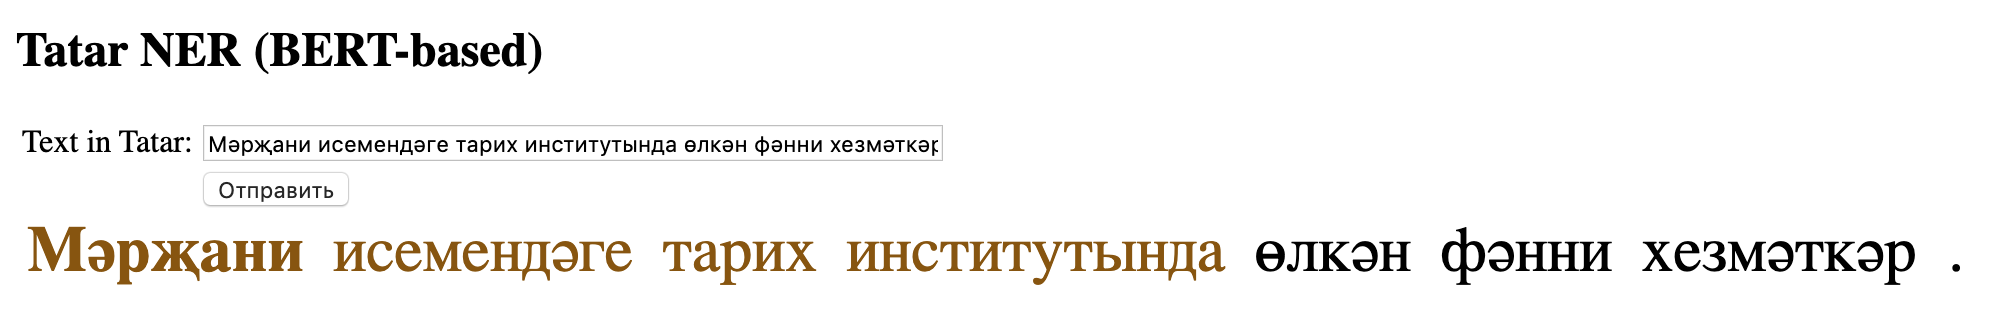
\includegraphics[width=\textwidth]{BERT_samp_1}
Всё распознано корректно, категория ORG
\label{fig:BERT_samp_1}
\end{figure}
\begin{figure}[H]
\caption{Зовут меня Ксения}
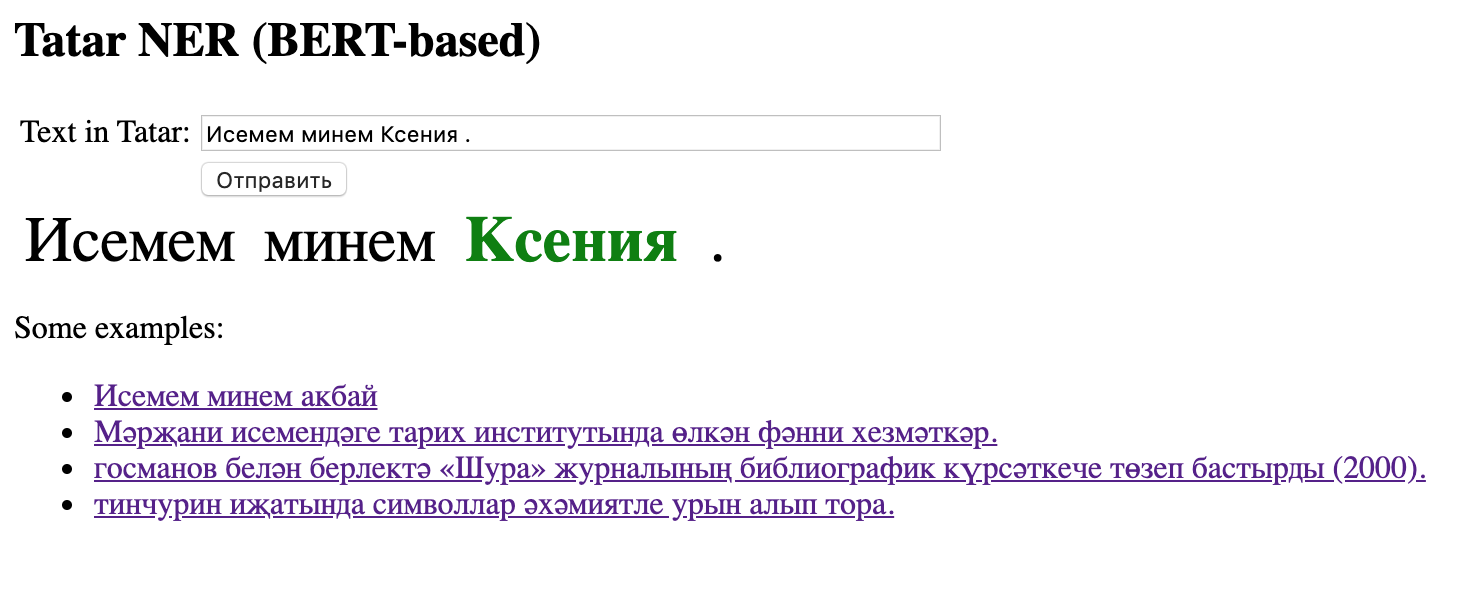
\includegraphics[width=\textwidth]{BERT_samp_2}
Всё распознано корректно, категория PER
\label{fig:BERT_samp_2}
\end{figure}
\begin{figure}[H]
\caption{Он решил изучать русский язык}
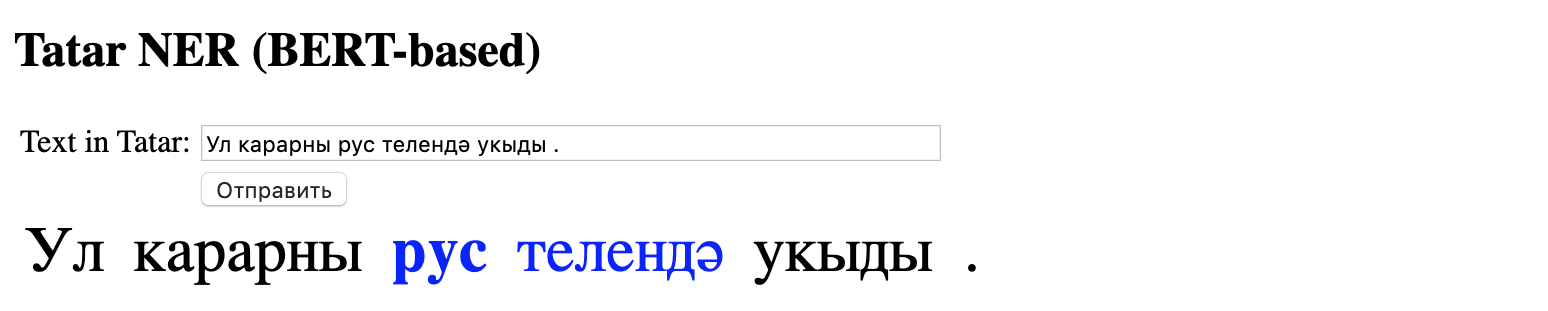
\includegraphics[width=\textwidth]{BERT_samp_3}
Всё распознано корректно, категория MISC
\label{fig:BERT_samp_3}
\end{figure}
\begin{figure}[H]
\caption{Празднование состоится в селе Асан Дюртюлинского района}
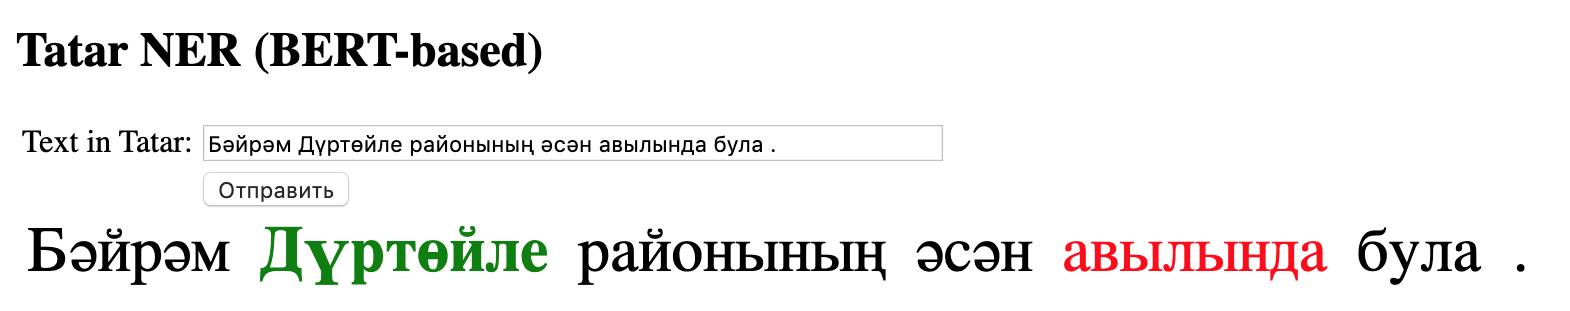
\includegraphics[width=\textwidth]{BERT_samp_4}
Не распознано имя села, хотя само понятие <<село>> распознано как категория LOC. <<Дюртюлиский>> ошибочно распознано как имя, <<район>> должно входить в название района.
\label{fig:BERT_samp_4}
\end{figure}



\section{Сравнение результатов}

Отдельной задачей стоял вопрос, как сравнить полученные результаты с предыдущими результатами в данной области. Было принято решение разметить некоторое количество предложений вручную, чтобы иметь качественные <<золотые>> данные, про которые было бы известно, что шанс неправильных меток в них гораздо ниже, чем в автоматически размеченных. Такая разметка была получена и следующим этапом воспроизведенный алгоритм Невзоровой, ВiLSTM-CRF и BERT (последние два обученные на датасете, основанном на Википедии) были запущены на этих данных. Теперь полученные результаты допустимо сравнивать между собой, поскольку они <<в равном положении>> и выполняют одинаковую задачу.

Результаты выполнения алгоритма Невзоровой с ручной фильтрацией на <<золотых>> данных приведены в таблице \ref{table:Nevzorova_res_1}


\begin{table}[h!]

\begin{tabular}{| l | l | l | l | l |}
\hline


 category &precision  &  recall & \textbf{f1-score} &  total\\
 \hline
 PER& 0.53&0.63&\textbf{0.58}& 374 \\
  \hline
 LOC& 0.50&0.05&\textbf{0.09}&  78 \\
  \hline
 ORG& 0.40&0.10&\textbf{0.15}&  21 \\ 
  \hline
 MISC& 0.83&0.62&\textbf{0.71}&   8 \\ 
 \hline
 \hline

 avg& 0.52&0.51&\textbf{0.48}& 481 \\
\hline
\end{tabular}

\caption{Результаты алгоритма Невзоровой}
\label{table:Nevzorova_res_1}
\end{table}

Результаты тестирования модели BERT на <<золотых>> данных приведены в таблице \ref{table:BERT_res_1}

\begin{table}[h!]

\begin{tabular}{| l | l | l | l | l |}
\hline

 category &precision  &  recall & \textbf{f1-score} &  total\\
\hline
PER &  0.53 & 0.60 & \textbf{0.56} &  374 \\ 
\hline
LOC &  0.50 & 0.05 & \textbf{0.09} &   78 \\ 
\hline
ORG &  0.33 & 0.10 & \textbf{0.15} &   21 \\
\hline
MISC &  0.56 & 0.62 & \textbf{0.59} &   8 \\
\hline
\hline

avg &  0.52 & 0.49 & \textbf{0.47} &  481 \\
\hline
\end{tabular}

\caption{Результаты модели BERT}
\label{table:BERT_res_1}
\end{table}

Результаты тестирования модели BiLSTM-CRF на <<золотых>> данных приведены в таблице \ref{table:BiLSTMCRF_res_1} пока таблицы нет, но скоро будет, и моё предположение таково, что он будет ещё хуже, чем BERT. Но даже если сравнимо, то точно не лучше, чем алгоритм Невзоровой.

\begin{table}[h!]

Тут будет таблица

\caption{Результаты модели Bi-LSTM-CRF}
\label{table:BiLSTMCRF_res_1}
\end{table}


Как видно из цифр выше, разметка данных с помощью алгоритма далеко не идеальная, и модели выучили ровно столько, сколько данные могли им дать (однако у меня была надежда, что модели выучат больше, чем им дали на вход; для этого они обучались на данных, которые не содержали в себе <<пустые>> предложения, чтобы не учить их определять данные без меток). 

%добавить сводную таблицу

\section{Выводы}

\begin{enumerate}
\item Воспроизведен алгоритм из статьи Невзоровой и др., он показал свою работоспособность и его можно использовать в дальнейшем. %ограничения
\item Получен набор n-грамм именованных сущностей и размеченный корпус, с которыми можно будет работать в дальнейшем.
\item Получены модели, предсказывающие именованные сущности, но результаты этих моделей из-за качества данных оставляют желать лучшего.
\item Текущие лучшие модели действительно работают хорошо и на татарском языке, обучаясь на данных настолько, насколько они это позволяют, но увы, ничего сверх этого получить от них не удалось. 
\item Всё зависит от того, насколько хорошо размечены данные, поэтому в будущих работах нужно лучше разметить данные, модели хорошо обучаются и на имеющемся количестве входных данных.
\end{enumerate}























